% !TeX root = ../../main.tex
\section{Mechanical drawings}
\label{app:reactor-drawings}
\subsection{3D mechanical design and engineering drawings}
\label{app:engineeringdesign}

\begin{figure}[H]
    \centering
    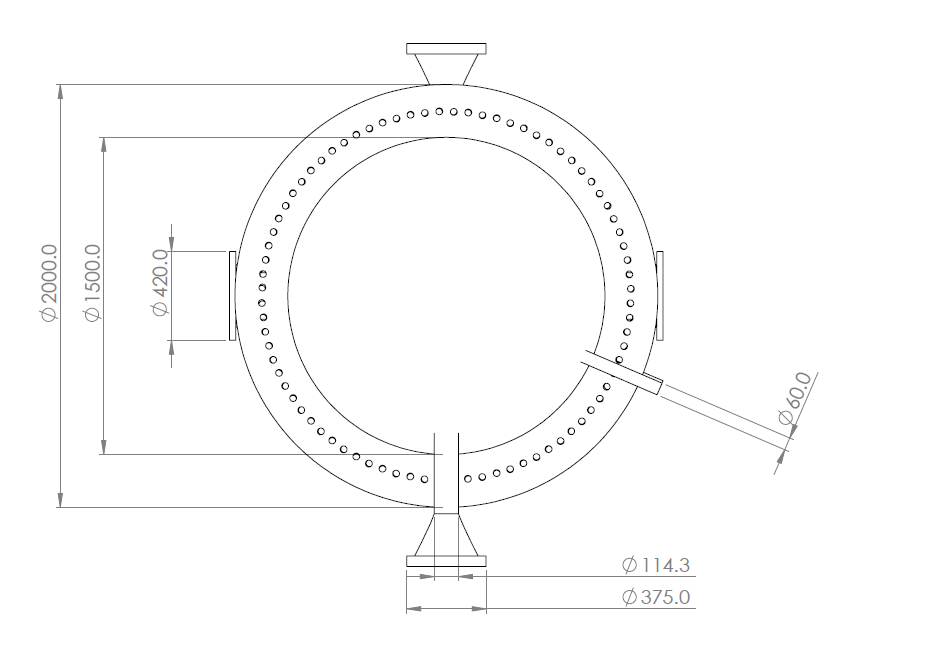
\includegraphics[width=0.6\linewidth]{chapters/2-reaction/figures/FYD reactor bottom view with calc.PNG}
    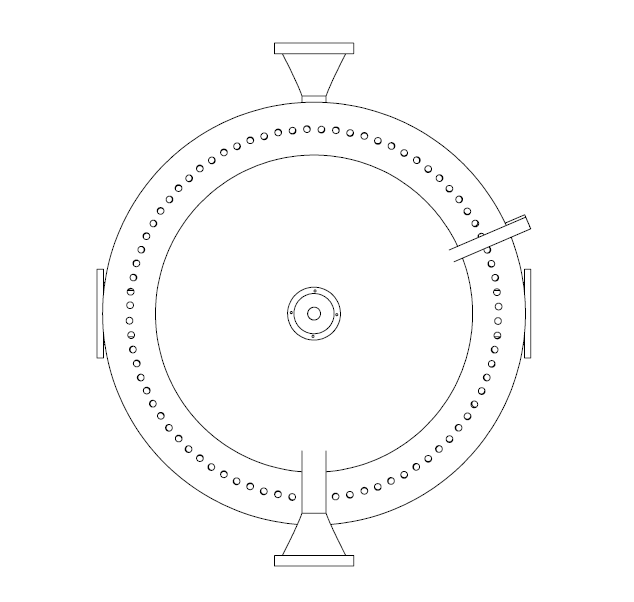
\includegraphics[width=0.45\linewidth]{chapters/2-reaction/figures/FYD reactor top view.PNG}
    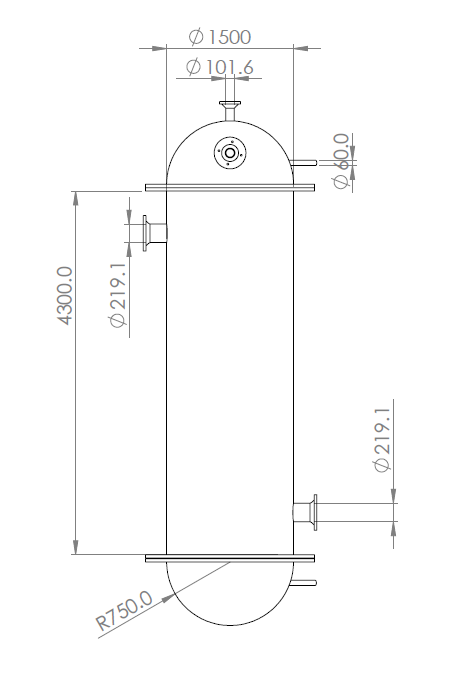
\includegraphics[width=0.49\linewidth]{chapters/2-reaction/figures/FYD reactor right view with calc.PNG}
    \caption{Top, bottom and right view of the reactor. All dimensions in units of mm}
    \label{fig:reactortopbottomrightview}
\end{figure}

\begin{figure}
    \centering
    \includegraphics{width=0.45\linewidth}
    \caption{Caption}
    \label{fig:my_label}
\end{figure}